		\begin{question}{N.A.}{Structure de molécules}{1}{}
			Quelle est la structure moléculaire de la molécule de \ce{H2O} dont une représentation est donnée ci-après?
			\begin{figure}
				\centering
				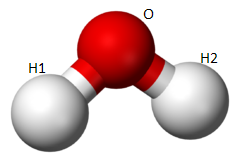
\includegraphics[height = 5cm]{Antoine/Figures_Antoine/240px-Water-3D-balls.png}
			\end{figure}
		\end{question}
		\begin{reponses}
			\item[false] Tétraédrique.
			\item[false] Cristalline cubique.
			\item[false] Linéaire.
			\item[true] En coude.
		\end{reponses}
		%%%%%%%%%%%%%%%%%%%%
		\begin{question}{N.A.}{Structure de molécules}{1}{}
			Quand on regarde par le dessus (selon la flèche rouge) une molécule d'eau \ce{H2O} dont une représentation est donnée ci-après, quelle figure observera-t-on?
			\begin{figure}
				\centering
				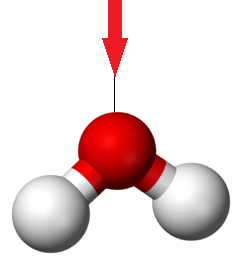
\includegraphics[height = 5cm]{Antoine/Figures_Antoine/240px-Water-3D-balls3.png}
			\end{figure}
		\end{question}
		\begin{reponses}
			\item[false] Un triangle dont les sommets sont les ombres des atomes composant la molécule.
			\item[true] Trois taches alignées formées par les ombres des atomes d'hydrogène, d'oxygène et d'hydrogène.
			\item[false] Un triangle équilatéral formé par l'ombre des trois atomes composant la molécules.
		\end{reponses}
		%%%%%%%%%%%%%%%%%%%%
		\begin{question}{N.A.}{Structure de molécules}{1}{}
			Quelle est la structure moléculaire de la molécule de \ce{CH4} dont une représentation est donnée ci-après?
			\begin{figure}
				\centering
				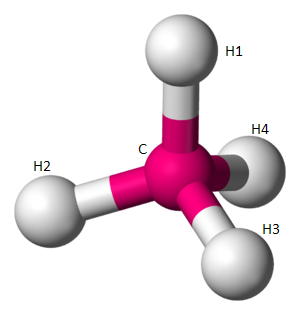
\includegraphics[height = 5cm]{Antoine/Figures_Antoine/300px-Tetrahedral-3D-balls.png}
			\end{figure}
		\end{question}
		\begin{reponses}
			\item[true] Tétraédrique.
			\item[false] Cristalline cubique.
			\item[false] Linéaire.
			\item[false] En diamant.
		\end{reponses}
		%%%%%%%%%%%%%%%%%%%%
		\begin{question}{N.A.}{Structure de molécules}{2}{}
			La molécule d'eau forme un coude au niveau de l'atome d'oxygène. L'angle $\widehat{\ce{H}_1\ce{O}\ce{H}_2}$ \SI{105}{\degree}. Quelle est alors la valeur de l'angle formé par l'atome d'oxygène et les atomes d'hydrogène (angle $\widehat{\ce{O}\ce{H}_1\ce{H}_2}$)?
			\begin{figure}
				\centering
				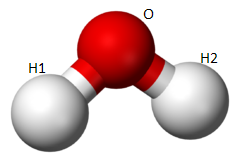
\includegraphics[height = 5cm]{Antoine/Figures_Antoine/240px-Water-3D-balls.png}
			\end{figure}
		\end{question}
		\begin{reponses}
			\item[true] \SI{37.5}{\degree}
				\item[false] \SI{45}{\degree}
				\item[false] \SI{105.5}{\degree}
				\item[false] \SI{20}{\degree}
		\end{reponses}
		%%%%%%%%%%%%%%%%%%%%
		\begin{question}{N.A.}{Structure de molécules}{2}{}
			La molécule \ce{CH4} forme un tétrahèdre dont l'atome de carbone est le centre. \SI{109}{\degree}. L'angle $\widehat{\ce{H}_1\ce{C}\ce{H}_2}$ vaut \SI{109}{\degree}. Que vaut alors l'angle $\widehat{\ce{C}\ce{H}_1\ce{H}_2}$?
			\begin{figure}
				\centering
				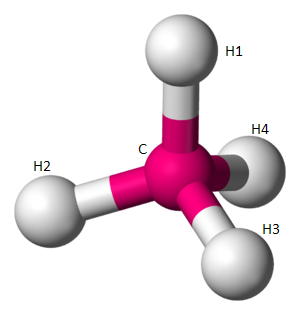
\includegraphics[height = 5cm]{Antoine/Figures_Antoine/300px-Tetrahedral-3D-balls.png}
			\end{figure}
		\end{question}
		\begin{reponses}
			\item[true] \SI{35.5}{\degree}
			\item[false] \SI{45}{\degree}
			\item[false] \SI{30.3}{\degree}
			\item[false] \SI{20.4}{\degree}
		\end{reponses}
		%%%%%%%%%%%%%%%%%%%%
		\begin{question}{N.A.}{Structure de molécules}{2}{}
			La molécule d'eau forme un coude dont l'atome d'oxygène est le centre. L'angle $\widehat{\ce{O}\ce{H}_1\ce{H}_2}$ vaut \SI{37.5}{\degree}. Quelle est alors la valeur de l'angle formé $\widehat{\ce{H}_1\ce{O}\ce{H}_2}$?
			\begin{figure}
				\centering
				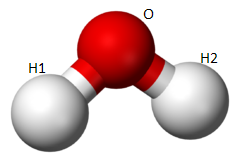
\includegraphics[height = 4cm]{Antoine/Figures_Antoine/240px-Water-3D-balls.png}
			\end{figure}
		\end{question}
			\begin{reponses}
			\item[true] \SI{105}{\degree}
			\item[false] \SI{45}{\degree}
			\item[false] \SI{100}{\degree}
			\item[false] \SI{20}{\degree}
			\end{reponses}
		%%%%%%%%%%%%%%%%%%%%
